\chapter{Étude 1 : Impact de l'Interactivité et de la Représentation sur l'Intérêt}
\label{ch:experimentation1}

% =============================================================================
% SECTION 4.1 : INTRODUCTION (TRANSITION DEPUIS CH3)
% =============================================================================
% Type C : Rédaction Originale
% Objectif : Liaison Ch3 (MemorIA) → Ch4 (Études contrôlées)
% =============================================================================

\section{Introduction}
\label{sec:exp1-introduction}

Le chapitre précédent a présenté la plateforme MemorIA, une infrastructure technique conçue pour déployer des agents conversationnels historiques en contexte scolaire. L'étude pilote exploratoire menée avec Jules César auprès d'élèves de sixième a fourni des observations qualitatives encourageantes : participation accrue d'élèves habituellement réservés, engagement spontané dans les échanges oraux, et réactions émotionnelles aux expressions faciales de l'agent. Ces résultats préliminaires suggéraient que l'interaction orale en temps réel avec un personnage historique virtuel pouvait susciter l'intérêt des élèves. Toutefois, la nature exploratoire de cette phase ne permettait pas d'isoler les mécanismes spécifiques à l'origine de ces réactions positives. Plusieurs facteurs se trouvaient confondus : la nouveauté du dispositif, l'interactivité orale, la représentation d'une figure historique, ou encore le style de communication adopté par l'agent.

Le présent chapitre inaugure la phase expérimentale contrôlée de cette recherche. Son objectif est de démêler l'influence respective de deux facteurs susceptibles d'affecter l'intérêt des élèves pour le contenu historique. Le premier facteur concerne la modalité d'interaction. Les observations pilotes suggéraient que la possibilité de questionner directement l'agent et d'obtenir des réponses immédiates favorisait l'intérêt. Cette intuition rejoint les travaux sur l'apprentissage actif, qui établissent que la participation directe des apprenants améliore leur motivation et leur traitement cognitif \citep{freeman2014active, deci2000intrinsic}. Il convenait donc de comparer systématiquement les conditions interactives, où les élèves dialoguent avec l'agent, aux conditions non interactives, où ils visionnent une présentation vidéo préenregistrée du même agent délivrant un contenu équivalent.

Le second facteur concerne l'alignement thématique entre l'identité de l'agent et le contenu pédagogique. La théorie de l'agence sociale postule que les indices sociaux dans les environnements d'apprentissage activent des réponses sociales chez les apprenants, favorisant un traitement cognitif plus profond \citep{moreno2001, mayer2012}. Un agent incarnant une figure historique liée au contenu de la leçon pourrait ainsi bénéficier d'un double effet : l'attrait pour une personnalité célèbre et la cohérence thématique entre le messager et le message. Cette hypothèse méritait d'être testée en comparant des agents historiques à des agents neutres présentant le même contenu dans un style exposé à la troisième personne.

Pour examiner ces deux facteurs, nous avons conçu une série de trois expérimentations adoptant un plan factoriel 2×2 (Interactivité × Alignement du personnage). Ce design permet d'évaluer les effets principaux de chaque facteur ainsi que leur interaction potentielle. Les trois études se distinguent par le niveau scolaire des participants, le personnage historique représenté, et le style de communication adopté par l'agent. Cette variation délibérée répond à un double objectif. D'une part, elle permet de tester la robustesse des effets observés à travers différents contextes développementaux, les élèves de sixième, quatrième et terminale présentant des profils cognitifs et des rapports à l'histoire distincts. D'autre part, elle offre l'opportunité d'explorer comment les caractéristiques de présentation de l'agent --- son ton, son registre de langue, sa propension à l'auto-divulgation --- modulent l'intérêt des élèves.

L'Expérimentation 1.1, menée avec des élèves de quatrième, mobilise Napoléon Bonaparte dans le cadre d'une leçon sur l'Empire français. Le personnage adopte un style formel et autoritaire, conforme à sa stature historique. L'Expérimentation 1.2, conduite avec des élèves de sixième, met en scène Jules César lors d'une séquence sur la République romaine. En réponse aux observations de la première étude, le style de communication a été ajusté : César se présente de manière plus accessible, partage ses doutes et ses expériences personnelles, et adopte un ton conversationnel ponctué d'humour. L'Expérimentation 1.3, réalisée avec des lycéens de terminale, compare Charles de Gaulle, figure d'autorité, à Louis, un jeune résistant fictif conçu comme une figure de pair. Cette dernière étude se concentre exclusivement sur les conditions interactives, les effets de l'interactivité ayant été établis dans les études précédentes.

Les mesures communes aux trois études portent sur l'intérêt des élèves, évalué à travers trois dimensions : l'intérêt pour l'activité d'apprentissage, l'intérêt pour le contenu de la leçon, et l'intérêt pour le personnage historique. Ces dimensions, adaptées de l'Inventaire de Motivation Intrinsèque \citep{deci1994facilitating} et alignées avec les travaux de \citet{hidi2006four} sur le développement de l'intérêt, permettent de capturer les différentes facettes de l'intérêt suscité par l'interaction avec l'agent.

Les sections suivantes présentent successivement chaque expérimentation, détaillant le contexte pédagogique, les conditions expérimentales, les participants, la procédure, les hypothèses, les résultats et leur discussion. Une section finale aborde les aspects transversaux de mise en œuvre technique et les considérations éthiques communes aux trois études.


% =============================================================================
% SECTION 4.2 : EXPÉRIMENTATION 1.1 - L'EMPIRE FRANÇAIS (4ÈME)
% =============================================================================

\section{Expérimentation 1.1 : L'Empire Français avec des élèves de 4\textsuperscript{ème}}
\label{sec:exp11}

\subsection{Contexte Pédagogique}
\label{subsec:exp11-contexte}

Cette première étude a été intégrée au programme de 4\textsuperscript{ème} portant sur l'Empire Français. Nous avons examiné deux facteurs susceptibles d'influencer l'intérêt des élèves pour le contenu historique. Premièrement, nous avons comparé les présentations interactives et non interactives. Les présentations vidéo non interactives offrent un contenu visuel et des éléments narratifs qui diffèrent des cours magistraux traditionnels. Les conditions interactives permettent aux élèves de dialoguer avec un agent virtuel, de poser des questions et de recevoir des réponses immédiates. Deuxièmement, nous avons examiné l'effet de l'alignement du personnage en comparant des agents historiques et neutres dans les conditions interactives et non interactives. Cette approche nous a permis d'étudier si l'alignement entre l'identité de l'agent et le contenu historique influence l'intérêt des élèves. Basée sur un plan expérimental inter-sujets, cette étude a mis en œuvre des conditions en classe pour maintenir la validité écologique.

\subsection{Conditions Expérimentales}
\label{subsec:exp11-conditions}

L'étude a employé un plan 2×2 inter-sujets avec deux variables indépendantes : l'Interactivité (Interactive vs. Non-Interactive) et l'alignement du personnage (Historique vs. Neutre). En utilisant Napoléon Bonaparte comme personnage historique, nous avons mesuré les effets de l'interactivité et de l'alignement du personnage sur trois dimensions d'intérêt : l'intérêt pour l'activité d'apprentissage, la figure historique et le contenu de la leçon. 

Dans les conditions interactives, les élèves ont participé à une conversation ouverte de 10 minutes avec l'agent virtuel généré par IA. L'agent a répondu aux questions, fourni des réponses contextuellement pertinentes et utilisé des expressions faciales et un ton vocal synchronisés pour transmettre des émotions. Dans les conditions non interactives, les élèves ont regardé une vidéo pré-enregistrée de 10 minutes de l'agent délivrant un monologue, avec des expressions faciales et un ton vocal synchronisés.

Pour l'alignement du personnage, la condition historique mettait en scène Napoléon Bonaparte parlant à la première personne, partageant des anecdotes personnelles et des expériences. La condition neutre, en revanche, présentait les mêmes informations historiques à travers un agent utilisant un style expositif, parlant à la troisième personne sans embellissement historique et utilisant des expressions plus sobres (voir Figure~\ref{fig:napoleon_conditions}).

\begin{figure}[htbp]
    \centering
    \includegraphics[width=0.8\textwidth]{images/ch4/napoleon_conditions.png}
    \caption{Comparaison des agents virtuels dans les conditions historique (Napoléon Bonaparte) et neutre de l'Expérimentation 1.1}
    \label{fig:napoleon_conditions}
\end{figure}

\subsection{Dispositif Expérimental}
\label{subsec:exp11-dispositif}

L'expérience s'est déroulée dans des salles de classe régulières, chacune équipée d'un ordinateur portable positionné sur le bureau de l'enseignant pour exécuter le système MemorIA. L'ordinateur portable, un Dell Precision 7780 avec un processeur Intel Core i7-1185G7, une carte graphique NVIDIA RTX 4090, 16 Go de RAM, avait deux dispositifs connectés : un haut-parleur de conférence Jabra Speak 750 pour capturer les demandes verbales des élèves, et une connexion au système d'affichage de la classe. Cette configuration permettait à toute la classe de voir et d'entendre simultanément l'agent virtuel pendant les sessions interactives. Pour les conditions non interactives, des vidéos pré-enregistrées ont été diffusées sur le même système. La taille de l'image projetée a été maintenue constante à travers les trois études, assurant la cohérence dans la présentation visuelle des agents virtuels.

\subsection{Participants}
\label{subsec:exp11-participants}

L'étude a impliqué un échantillon de 113 élèves de 4\textsuperscript{ème} (59 filles, 54 garçons ; âge : M = 13,2 ans, ET = 0,8, étendue : 12-14 ans) recrutés dans un collège français. Les participants ont été recrutés dans quatre classes, résultant en environ 30 élèves par classe.

Le protocole d'étude a été examiné et approuvé par le comité d'éthique institutionnel. Les parents et les élèves ont reçu des informations détaillées sur l'étude et ont été informés que la participation était volontaire. Un consentement écrit a été obtenu des parents/tuteurs légaux, et les élèves ont fourni un assentiment écrit. Seuls les élèves ayant retourné les deux formulaires ont participé à l'expérience. Tout au long du processus, les participants ont été assurés de leur droit à la confidentialité et de leur liberté de se retirer de l'étude.

\subsection{Procédure}
\label{subsec:exp11-procedure}

L'expérience a été intégrée dans une leçon d'histoire régulière de 60 minutes dans des conditions « écologiques » authentiques. En arrivant dans la salle de classe, l'enseignant a accueilli et présenté les expérimentateurs aux élèves. Après que les expérimentateurs ont expliqué les activités prévues, tous les participants ont complété un questionnaire initial évaluant leur intérêt pour l'activité d'apprentissage, la figure historique et le contenu de la leçon. 

Les classes ont été assignées aléatoirement à l'une des quatre conditions expérimentales. Dans les conditions interactives, les élèves ont été informés qu'ils interagiraient avec un agent virtuel, représentant soit une figure historique soit un personnage neutre. Les élèves ont travaillé en petits groupes de 3-4 pour générer collaborativement des questions liées au sujet de la leçon. Chaque groupe a sélectionné un porte-parole qui s'est engagé avec l'agent virtuel (personnifiant soit Napoléon Bonaparte soit un personnage neutre) pendant environ 2 minutes. Les réponses parlées de l'agent, accompagnées d'expressions faciales appropriées, ont été affichées sur un grand écran avec l'audio diffusé à travers les haut-parleurs de la classe, permettant à toute la classe d'observer chaque interaction.

Dans les conditions non interactives, les participants ont visionné une vidéo pré-enregistrée de 10 minutes de l'agent virtuel (figure historique ou neutre) délivrant un monologue sur sa vie et ses expériences, se concentrant sur des sujets liés au contenu de la leçon (voir Figure~\ref{fig:classroom_napoleon}).

\begin{figure}[htbp]
    \centering
    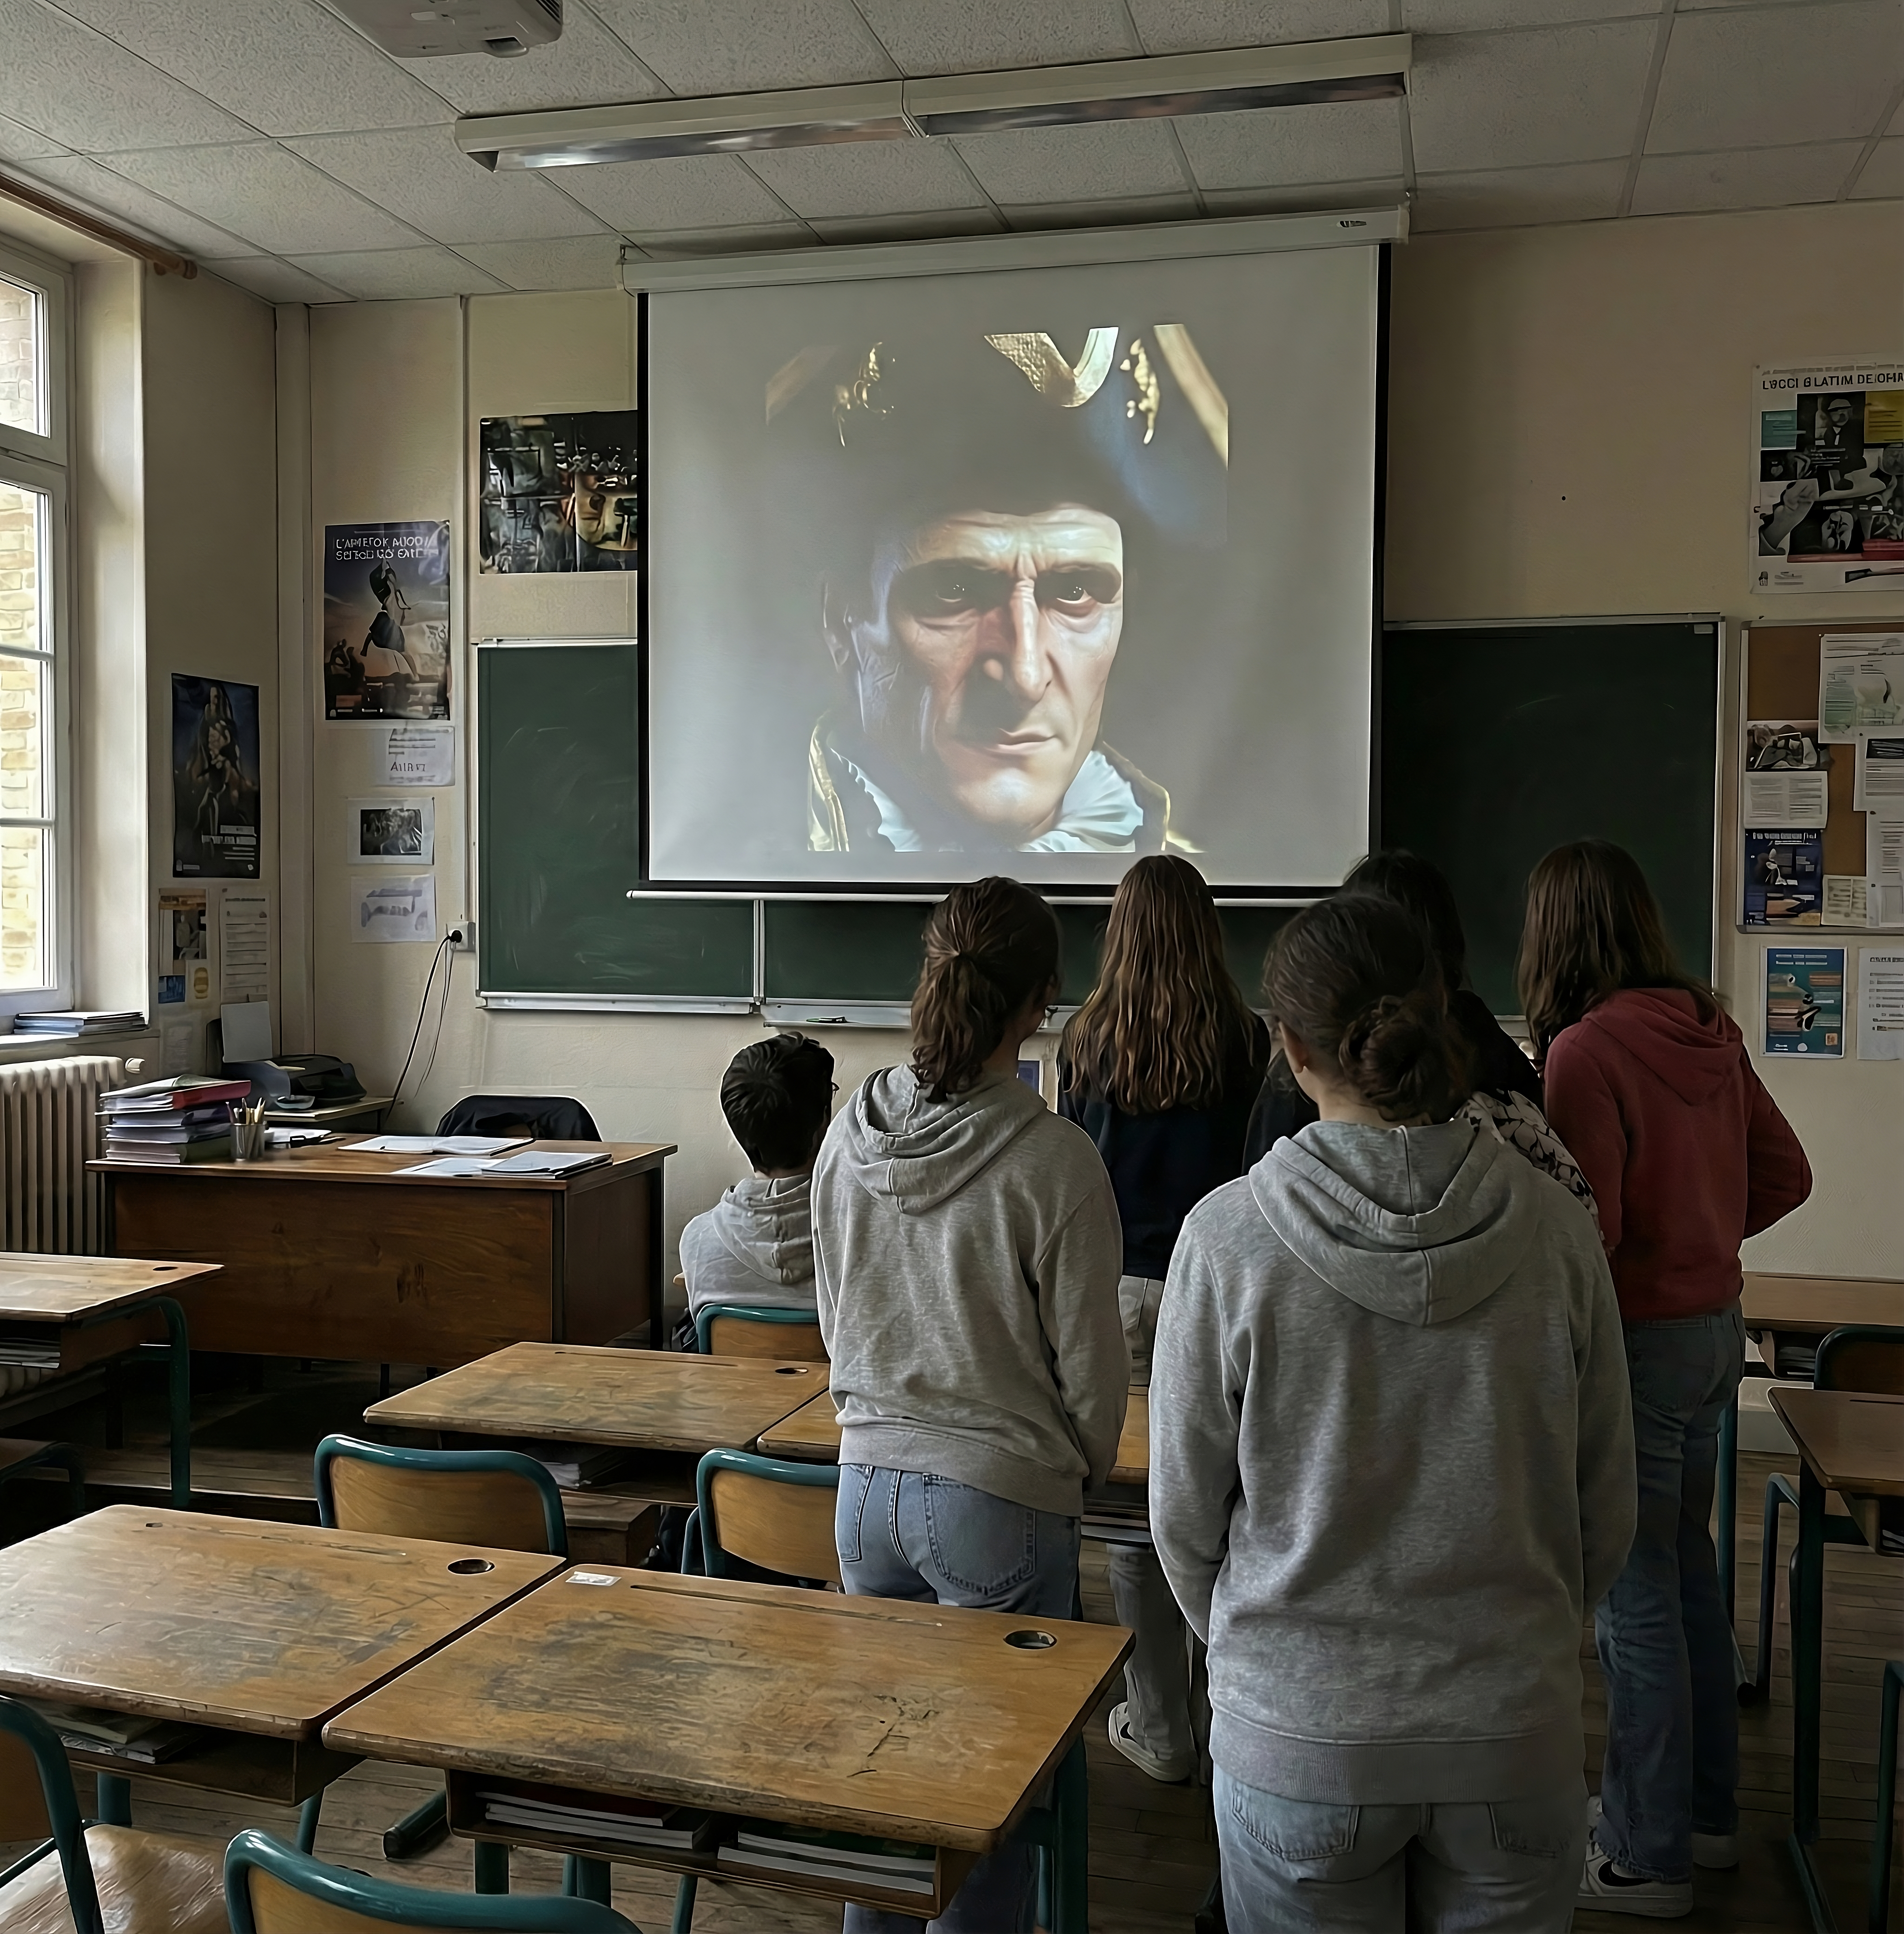
\includegraphics[width=0.8\textwidth]{images/ch4/classroom_napoleon.png}
    \caption{Configuration de la classe pendant l'Expérimentation 1.1 avec Napoléon Bonaparte}
    \label{fig:classroom_napoleon}
\end{figure}

Suite à la phase expérimentale, les participants ont complété un questionnaire post-expérience évaluant les mêmes trois dimensions d'intérêt. Des discussions de groupe ont ensuite été facilitées avec chaque classe, fournissant un forum ouvert pour que les participants partagent leurs réflexions sur leurs interactions avec les agents virtuels. Nous avons souligné que les agents virtuels étaient des représentations générées par IA, et l'enseignant a eu l'opportunité de clarifier et de corriger toute inexactitude historique qui a émergé pendant les interactions. Au cours de ces discussions, les participants ont exploré des questions sur l'authenticité historique et les implications de l'utilisation de l'IA dans des contextes éducatifs.

\subsection{Mesures}
\label{subsec:exp11-mesures}

L'intérêt a été évalué à l'aide de questionnaires adaptés de l'Inventaire de Motivation Intrinsèque (IMI) \citep{deci1994facilitating} et alignés avec les travaux de \citet{hidi2006four} sur le développement de l'intérêt situationnel et individuel.

Trois dimensions ont été mesurées : l'intérêt pour l'activité d'apprentissage (plaisir, valeur et volonté de s'engager), l'intérêt pour la figure historique (curiosité et désir d'en apprendre davantage sur le personnage), et l'intérêt pour le contenu de la leçon (engagement et curiosité concernant l'Empire Français). Chaque dimension a été évaluée à travers trois items distincts de questionnaire. Les questions ont été notées sur des échelles à 7 points allant de 1 (fortement en désaccord) à 7 (fortement en accord). Pour minimiser les effets d'ordre et les biais de réponse, les items ont été entièrement randomisés à travers toutes les dimensions. Les réponses au questionnaire pré-expérience, mesurant l'intérêt initial pour l'activité d'apprentissage, la figure historique et le contenu de la leçon, ont été utilisées comme covariables dans les analyses pour contrôler les différences individuelles dans l'intérêt de base.

\subsection{Hypothèses}
\label{subsec:exp11-hypotheses}

Basées sur notre revue de la littérature et le design de notre étude, nous avons proposé les hypothèses suivantes :

\textbf{H1 :} Les participants dans les conditions interactives présenteront un intérêt post-intervention plus élevé pour l'activité d'apprentissage (H1.1), le contenu de la leçon (H1.2), et le personnage historique (H1.3) comparé à ceux dans les conditions non interactives, après contrôle des niveaux d'intérêt pré-intervention.

Cette hypothèse est fondée sur les bénéfices pédagogiques établis de l'apprentissage actif et de l'interactivité \citep{freeman2014active, moreno2007interactive}. L'engagement des élèves, facilité par le dialogue et le contrôle du rythme d'apprentissage, est suggéré comme étant un facteur clé dans la promotion de la motivation intrinsèque et de l'apprentissage profond \citep{deci2000intrinsic}. Des recherches récentes indiquent que les interactions conversationnelles avec des agents pédagogiques peuvent améliorer significativement l'engagement et l'intérêt des apprenants \citep{hidi2006four}. L'impact positif des agents virtuels interactifs alimentés par l'IA sur divers résultats d'apprentissage \citep{pataranutaporn2023, prasongpongchai2024} s'aligne avec les théories de l'apprentissage multimédia mettant l'accent sur l'importance de la communication bidirectionnelle pour un traitement cognitif efficace \citep{moreno2007interactive}. L'accent mis sur l'autonomie de l'apprenant et l'exploration active inhérent aux conditions interactives s'aligne avec les principes fondamentaux de l'apprentissage actif. Des études en enseignement de l'histoire, explorant les récits numériques interactifs \citep{petousi2022} et l'engagement émotionnel avec le contenu historique \citep{roussou2024}, suggèrent en outre que la participation active, plutôt que la réception passive \citep{deslauriers2019}, peut contribuer à une compréhension et un intérêt accrus pour l'histoire.

\textbf{H2 :} Les participants dans les conditions de figure historique présenteront un intérêt post-intervention plus élevé pour l'activité d'apprentissage (H2.1), le contenu de la leçon (H2.2), et le personnage historique (H2.3) comparé à ceux dans les conditions de figure neutre, après contrôle des niveaux d'intérêt pré-intervention.

Cette hypothèse est basée sur la théorie de l'agence sociale \citep{moreno2001, mayer2012}, qui postule que les signaux sociaux dans les environnements d'apprentissage peuvent activer des réponses sociales chez les apprenants, conduisant à un traitement cognitif plus profond. La représentation de figure historique peut influencer l'intérêt des élèves par deux mécanismes : premièrement, en impliquant l'interaction avec des personnalités célèbres et potentiellement admirées \citep{pataranutaporn2022}, car ces figures historiques sont des personnages bien connus de l'histoire nationale, et deuxièmement, par l'alignement thématique entre la figure historique et le contenu de la leçon. En effet, \citet{schmidt2019} ont démontré que l'alignement thématique améliore l'expérience utilisateur en rendant les interactions plus attrayantes et stimulantes. Cet alignement peut ainsi affecter la pertinence perçue du matériel d'apprentissage par les élèves. Cette prédiction s'aligne avec la théorie du développement de l'intérêt \citep{hidi2006, harackiewicz2016}, qui distingue entre l'intérêt situationnel déclenché et l'intérêt situationnel maintenu. Les dialogues interactifs avec des figures historiques peuvent déclencher un intérêt initial par des éléments nouveaux et inattendus dans l'interaction, tandis que la connexion personnelle établie par le questionnement direct peut aider à maintenir cet intérêt \citep{renninger2015}. Comme \citet{harackiewicz2016} l'ont démontré, les environnements d'apprentissage qui combinent des caractéristiques déclenchantes avec des opportunités d'engagement significatif peuvent soutenir la transition de l'attention momentanée vers un intérêt soutenu. En permettant aux élèves d'explorer le contenu historique par des interactions personnalisées, notre approche peut combler le fossé entre les événements historiques et la curiosité personnelle des élèves, un facteur clé dans le développement de l'intérêt \citep{hidi2020}.

\subsection{Résultats}
\label{subsec:exp11-resultats}

Nous avons conduit des analyses de covariance bidirectionnelles (ANCOVA) pour chaque variable dépendante (intérêt pour l'activité d'apprentissage [Post\_Act], intérêt pour le contenu de la leçon [Post\_Les], et intérêt pour le personnage historique [Post\_Char]), avec l'interactivité et l'alignement du personnage comme variables indépendantes et les mesures pré-intervention correspondantes comme covariables. Cette approche nous a permis de contrôler les différences préexistantes entre les participants tout en testant nos hypothèses sur les effets de l'interactivité et de l'alignement du personnage sur l'intérêt des élèves. Des analyses préliminaires ont été conduites pour vérifier que les hypothèses de l'ANCOVA étaient satisfaites, et des corrections ont été appliquées lorsque nécessaire pour ajuster les violations d'homogénéité de variance. Les données qualitatives issues des discussions de groupe post-intervention ont complété nos analyses quantitatives, fournissant une compréhension plus complète des mécanismes psychologiques sous-jacents aux effets observés.

Avant d'analyser les effets de nos variables indépendantes, nous avons vérifié la comparabilité initiale des groupes expérimentaux. Des tests de Mann-Whitney ont comparé les scores d'intérêt initiaux entre les conditions d'interactivité (Vidéo vs. Interactive) et d'alignement du personnage (Neutre vs. Historique). Aucune différence significative n'a été trouvée entre les groupes Vidéo et Interactif, ni entre les groupes Neutre et Historique, démontrant une bonne comparabilité initiale. Ces résultats supportent la validité de nos analyses subséquentes, car ils démontrent que les effets observés ne peuvent être attribués à des différences préexistantes entre les groupes.

Aucun effet d'interaction significatif entre l'interactivité et l'alignement du personnage n'a été observé pour aucune des mesures d'intérêt (Post\_Act : F(1, 108) = 1,399, p = ,240, $\eta^2$ = ,010 ; Post\_Les : F(1, 108) = 0,457, p = ,501, $\eta^2$ = ,002 ; Post\_Char : F(1, 108) = 1,336, p = ,250, $\eta^2$ = ,007). 

Un effet principal de l'interactivité a été observé sur l'intérêt pour l'activité d'apprentissage (Post\_Act ; F(1, 108) = 23,547, p < ,001, $\eta^2$ = ,166), tandis que l'alignement du personnage n'a montré aucun effet significatif (F(1, 108) = 2,269, p = ,135, $\eta^2$ = ,016). Les élèves dans les conditions interactives ont rapporté un intérêt plus élevé (M = 5,699, ET = 1,133 pour le personnage historique ; M = 5,844, ET = 1,176 pour le personnage neutre) comparé à ceux dans les conditions vidéo (M = 4,226, ET = 1,513 pour le personnage historique ; M = 4,960, ET = 1,338 pour le personnage neutre).

\begin{figure}[htbp]
    \centering
    \includegraphics[width=0.6\textwidth]{images/ch4/napoleon_post_act.png}
    \caption{Intérêt des élèves de 4\textsuperscript{ème} pour l'activité d'apprentissage (Post\_Act) en fonction de l'interactivité et de l'alignement du personnage. Les barres d'erreur représentent les écarts-types}
    \label{fig:napoleon_post_act}
\end{figure}

Pour l'intérêt pour le contenu de la leçon (Post\_Les), un effet principal de l'interactivité a été trouvé (F(1, 108) = 11,231, p = ,001, $\eta^2$ = ,052), sans effet significatif de l'alignement du personnage (F(1, 108) = 1,377, p = ,243, $\eta^2$ = ,006). Les scores d'intérêt étaient plus élevés dans les conditions interactives (M = 5,455, ET = 1,218 pour le personnage neutre ; M = 4,789, ET = 1,198 pour le personnage historique) comparé aux conditions vidéo (M = 4,500, ET = 1,375 pour le personnage historique ; M = 5,160, ET = 1,265 pour le personnage neutre).

\begin{figure}[htbp]
    \centering
    \includegraphics[width=0.6\textwidth]{images/ch4/napoleon_post_les.png}
    \caption{Intérêt des élèves de 4\textsuperscript{ème} pour le contenu de la leçon (Post\_Les) en fonction de l'interactivité et de l'alignement du personnage. Les barres d'erreur représentent les écarts-types}
    \label{fig:napoleon_post_les}
\end{figure}

De manière similaire, pour l'intérêt pour le personnage historique (Post\_Char), l'analyse a révélé un effet principal de l'interactivité (F(1, 108) = 5,901, p = ,017, $\eta^2$ = ,030), sans effet significatif de l'alignement du personnage (F(1, 108) = 0,337, p = ,563, $\eta^2$ = ,002). Les conditions interactives ont montré un intérêt plus élevé (M = 5,655, ET = 1,153 pour le personnage neutre ; M = 5,033, ET = 1,198 pour le personnage historique) comparé aux conditions vidéo (M = 4,904, ET = 1,323 et M = 4,906, ET = 1,346 respectivement).

\begin{figure}[htbp]
    \centering
    \includegraphics[width=0.6\textwidth]{images/ch4/napoleon_post_char.png}
    \caption{Intérêt des élèves de 4\textsuperscript{ème} pour le personnage historique (Post\_Char) en fonction de l'interactivité et de l'alignement du personnage. Les barres d'erreur représentent les écarts-types}
    \label{fig:napoleon_post_char}
\end{figure}

\subsection{Discussion}
\label{subsec:exp11-discussion}

Notre analyse a révélé des patterns spécifiques concernant les effets de l'interactivité sur l'intérêt des élèves, tandis que l'alignement du personnage n'a montré aucune influence claire. Pour notre première hypothèse (H1), l'interactivité a démontré une influence positive significative sur l'intérêt des élèves. Les élèves qui participent à des dialogues avec des agents virtuels rapportent des niveaux d'intérêt plus élevés pour l'activité d'apprentissage (Post\_Act), le contenu de la leçon (Post\_Les) et le personnage historique (Post\_Char) comparés à ceux qui visionnent des vidéos non interactives. Ces résultats s'alignent avec la recherche sur les interactions avec des agents virtuels alimentés par l'IA \citep{prasongpongchai2024, pataranutaporn2023}. Notre seconde hypothèse (H2) prédisait un intérêt plus élevé pour le personnage historique, mais les données n'ont révélé aucune différence significative. Alors que des recherches antérieures suggéraient des bénéfices de l'alignement thématique pour l'intérêt dans les interactions virtuelles, nos résultats indiquent qu'un tel alignement nécessite des considérations additionnelles pour favoriser efficacement l'intérêt. Notre choix de perspective narrative pour Napoléon mérite une attention particulière. En faisant partager à Napoléon ses expériences et ses pensées directement, nous anticipions que cette approche créerait une connexion plus immédiate avec les élèves. La recherche de \citet{kim2020} suggère que la narration directe peut réduire la distance psychologique, même avec des personnages perçus comme différents de soi. Cependant, les résultats de \citet{wimmer2021} indiquent que la perspective narrative seule ne garantit pas une connexion améliorée. Dans notre cas, les retours qualitatifs révèlent que les élèves ont perçu la narration de Napoléon comme distante, caractérisée par un langage formel qui a créé des barrières plutôt que des opportunités de connexion. Le langage élevé et le ton autoritaire ont pu contribuer à cette perception de distance. Cet intérêt limité pourrait être mieux compris à travers les travaux de \citet{linsiegler2016} sur la façon dont les élèves se connectent avec des figures éminentes. Leur recherche a révélé que les élèves s'engagent plus profondément lorsqu'ils rencontrent les luttes et les défis des figures historiques plutôt que simplement leurs accomplissements, suggérant que notre représentation a pu amplifier la distance perçue entre leurs expériences et les siennes. Le personnage neutre, non contraint par une telle formalité, semble fournir un point d'entrée plus accessible au contenu. Cela s'aligne avec la recherche de \citet{lin2020} mettant en évidence comment le style conversationnel peut impacter significativement l'intérêt dans des contextes éducatifs. Le contexte développemental des élèves de 4\textsuperscript{ème} apparaît pertinent pour ces résultats. Les adolescents à ce stade expérimentent des capacités cognitives en évolution \citep{inhelder1958}. Les travaux de \citet{calvert2020} sur la confiance et la connexion émotionnelle dans les interactions virtuelles suggèrent que ces facteurs influencent particulièrement la façon dont l'intérêt se développe pendant l'adolescence. Le style de présentation formel ne s'aligne pas de manière optimale avec les besoins des élèves à ce stade développemental. Ces résultats de l'Étude 1 informent notre approche subséquente de la conception de personnages. Plutôt que d'écarter le potentiel de l'alignement de personnage historique, nous identifions des opportunités d'ajuster le style de présentation tout en maintenant l'authenticité historique.


% =============================================================================
% SECTION 4.3 : EXPÉRIMENTATION 1.2 - L'EMPIRE ROMAIN (6ÈME)
% =============================================================================

\section{Expérimentation 1.2 : L'Empire Romain avec des élèves de 6\textsuperscript{ème}}
\label{sec:exp12}

\subsection{Contexte Pédagogique et Choix du Personnage}
\label{subsec:exp12-contexte}

En réponse aux observations de la première étude, nous avons apporté des modifications importantes à notre approche pour l'étude suivante avec des élèves de 6\textsuperscript{ème}. Nous avons sélectionné Jules César comme figure historique en raison de sa forte présence dans la culture populaire française, notamment à travers les bandes dessinées Astérix. Les élèves de 6\textsuperscript{ème} (10-12 ans) sont familiers avec César à travers ces médias, potentiellement créant une connexion plus accessible que Napoléon pour les élèves de 4\textsuperscript{ème}. 

De plus, nous avons adapté le style de présentation et le conditionnement du personnage de César pour créer une persona plus empathique et accessible. Contrairement au ton formel et autoritaire de Napoléon, le personnage de César a été développé avec :

\begin{itemize}
\item Un accent sur la vulnérabilité et les expériences personnelles
\item Des reconnaissances de doutes et d'anxiétés
\item Un style conversationnel décontracté, avec des blagues occasionnelles et des réponses ludiques
\end{itemize}

Par exemple, lors de la discussion de campagnes militaires, César a été incité à partager non seulement des décisions stratégiques mais aussi des expériences personnelles : « Je me souviens d'avoir ressenti de l'anxiété la nuit avant la bataille, tout comme vous pourriez vous sentir avant un test important. » Plutôt que de maintenir une rigueur historique stricte, ce qui serait spéculatif étant donné la documentation limitée de la personnalité de César, nous avons priorisé la création d'interactions engageantes qui résonneraient avec des élèves de 6\textsuperscript{ème}. La synthèse vocale et l'animation faciale ont été ajustées en conséquence, incorporant des expressions plus variées et des changements tonaux pour soutenir cette caractérisation. Ces modifications ont été mises en œuvre tout en maintenant les paramètres techniques de base de l'Étude 1 (température : 0,7, longueur de réponse : 150 tokens, pénalité de présence : 0,5).

\subsection{Conditions Expérimentales et Plan}
\label{subsec:exp12-conditions}

Le plan expérimental a reflété celui de l'Étude 1, employant un plan inter-sujets 2×2 avec les mêmes variables indépendantes : Interactivité (Interactive vs. Non-Interactive) et alignement du personnage (Historique vs. Neutre). Les quatre conditions expérimentales étaient identiques à la première étude, Jules César remplaçant Napoléon Bonaparte (voir Figure~\ref{fig:caesar_conditions}).

\begin{figure}[htbp]
    \centering
    \includegraphics[width=0.8\textwidth]{images/ch4/caesar_conditions.png}
    \caption{Comparaison des agents virtuels dans les conditions historique (Jules César) et neutre de l'Expérimentation 1.2}
    \label{fig:caesar_conditions}
\end{figure}

\subsection{Dispositif Expérimental}
\label{subsec:exp12-dispositif}

La configuration expérimentale est restée inchangée, l'étude étant menée dans des salles de classe régulières équipées d'un ordinateur portable et d'un système de projection. Le même haut-parleur de conférence a été utilisé pour l'entrée et la sortie audio, assurant la cohérence dans l'environnement technologique à travers les études.

\subsection{Participants}
\label{subsec:exp12-participants}

La deuxième étude a impliqué un échantillon de 113 élèves de 6\textsuperscript{ème} (61 filles, 52 garçons ; âge : M = 11,2 ans, ET = 0,7, étendue : 10-12 ans) recrutés dans le même collège français. L'étude a suivi les mêmes directives éthiques que la première étude, assurant la participation volontaire et le consentement éclairé des élèves et de leurs parents/tuteurs.

\subsection{Procédure}
\label{subsec:exp12-procedure}

L'expérience a suivi le protocole de l'Étude 1. L'expérience s'est déroulée dans le cadre d'une seule leçon d'histoire de 60 minutes. Les participants ont d'abord complété un questionnaire initial évaluant leur intérêt pour le sujet de la leçon (la Guerre des Gaules), la figure historique (Jules César ou personnage neutre), et l'activité d'apprentissage. Les classes ont été assignées aléatoirement à l'une des quatre conditions expérimentales. Dans les conditions interactives, les élèves ont été informés qu'ils interagiraient avec un agent virtuel, représentant soit Jules César soit un personnage neutre. Les élèves ont travaillé en petits groupes de 3-4 pour générer collaborativement des questions sur la leçon. Chaque groupe a sélectionné un porte-parole qui s'est engagé avec l'agent virtuel pendant environ 2 minutes. Les réponses de l'agent ont été affichées sur un grand écran, permettant à toute la classe d'observer les interactions. Avec 8-10 groupes par classe, l'activité totale a duré environ 20 minutes.

Dans les conditions non interactives, les participants ont visionné une vidéo pré-enregistrée de 10 minutes de l'agent virtuel (Jules César ou figure neutre) discutant de moments clés de l'histoire romaine : sa carrière d'enseignement précoce, son alliance politique avec Pompée, le Premier Triumvirat, les Guerres des Gaules, et les événements ayant conduit à son assassinat (voir Figure~\ref{fig:classroom_caesar}). Suite à la phase expérimentale, les participants ont complété un questionnaire post-expérience et ont participé à des discussions de groupe où les élèves ont partagé leurs expériences et l'enseignant a eu l'opportunité d'adresser toute inexactitude historique.

\begin{figure}[htbp]
    \centering
    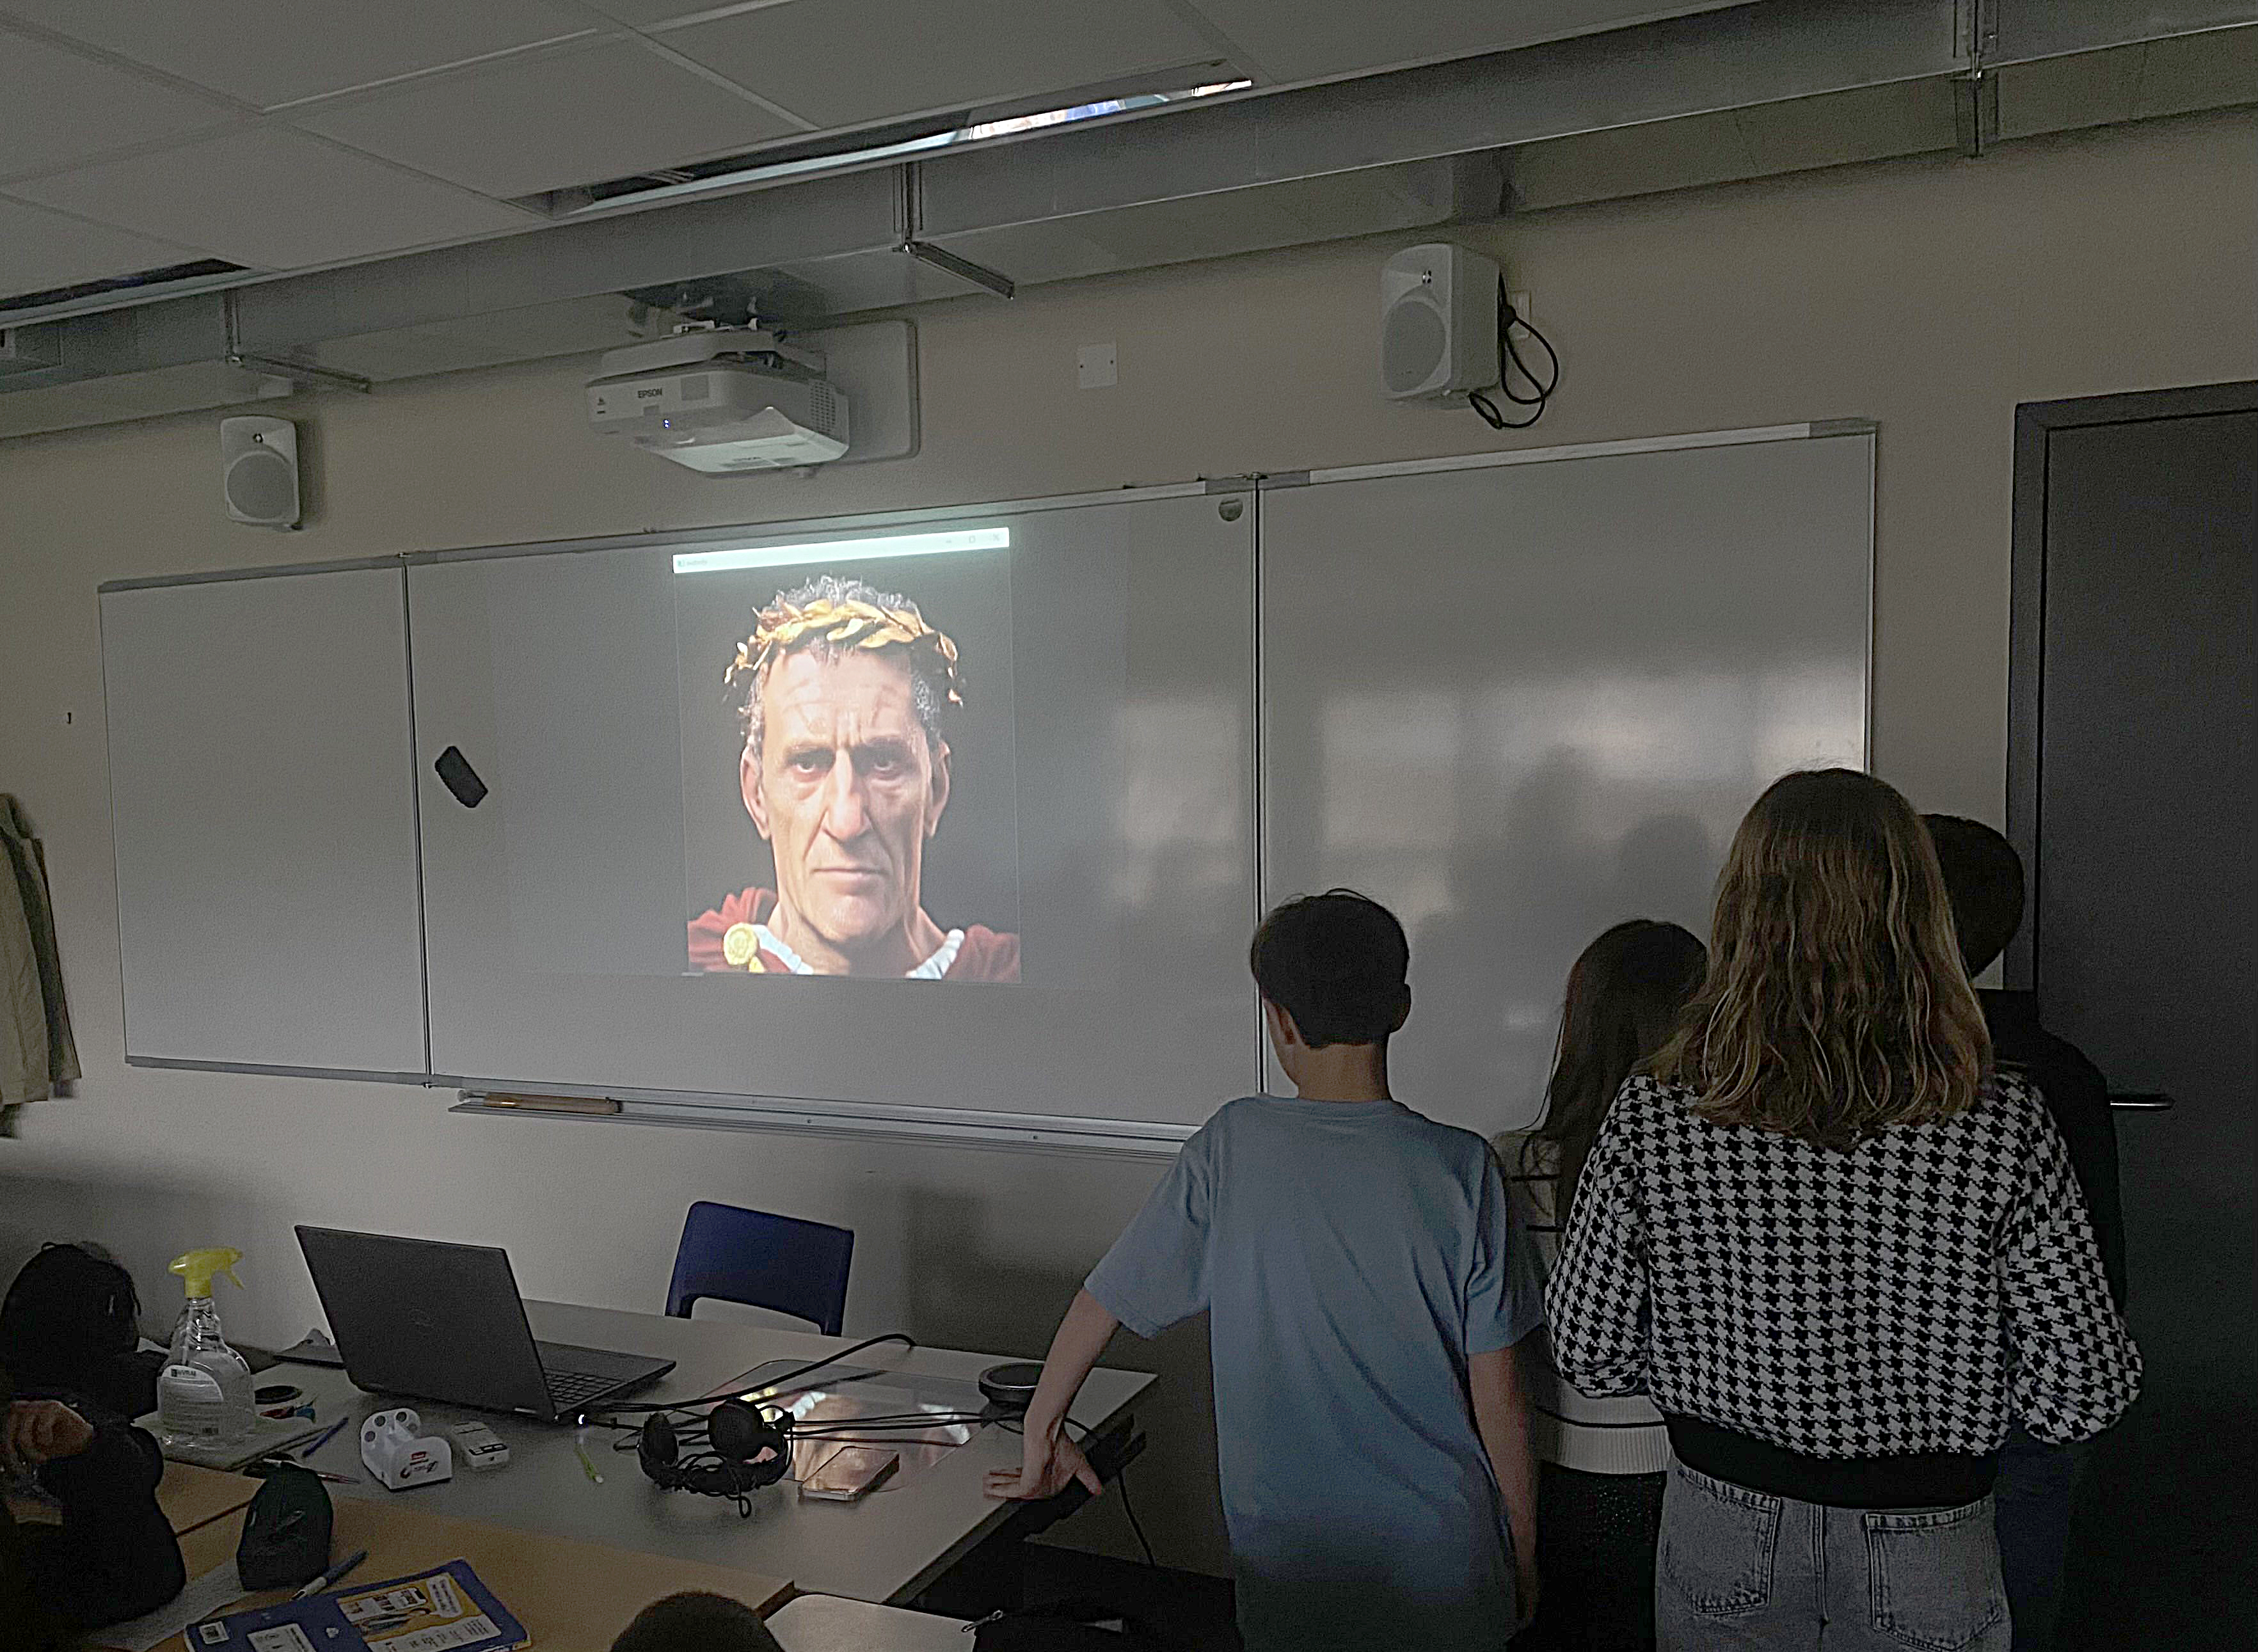
\includegraphics[width=0.8\textwidth]{images/ch4/classroom_caesar.png}
    \caption{Élèves de 6\textsuperscript{ème} interagissant avec Jules César pendant l'Expérimentation 1.2. Les élèves ont travaillé en petits groupes pour générer des questions, avec des porte-paroles engageant des dialogues de 2 minutes avec l'agent virtuel projeté sur grand écran}
    \label{fig:classroom_caesar}
\end{figure}

\subsection{Mesures}
\label{subsec:exp12-mesures}

Les mesures d'intérêt ont été maintenues cohérentes avec l'Étude 1, utilisant des questionnaires adaptés de l'IMI \citep{deci1994facilitating} et alignés avec les travaux de \citet{hidi2006four} sur le développement de l'intérêt situationnel et individuel. Les trois dimensions mesurées étaient l'intérêt pour l'activité d'apprentissage (Post\_Act), l'intérêt pour la figure historique (Post\_Char), et l'intérêt pour le contenu de la leçon (Post\_Les). Chaque dimension a été évaluée à travers trois items notés sur des échelles à 7 points. Les réponses au questionnaire initial ont été utilisées comme covariables dans les analyses pour contrôler les différences d'intérêt de base.

\subsection{Hypothèses}
\label{subsec:exp12-hypotheses}

Pour l'Étude 2, nous avons maintenu les hypothèses concernant les effets de l'interactivité (H1) et de l'alignement du personnage (H2) sur l'intérêt des élèves. Ces hypothèses ont continué à guider notre investigation sur comment ces facteurs influencent l'intérêt des élèves pour le contenu historique.

\subsection{Résultats}
\label{subsec:exp12-resultats}

Les effets de l'interactivité et de l'alignement du personnage sur les trois dimensions d'intérêt sont illustrés dans les Figures~\ref{fig:caesar_post_act}, \ref{fig:caesar_post_les}, et \ref{fig:caesar_post_char}. Les ANCOVA n'ont révélé aucun effet d'interaction significatif entre l'interactivité et l'alignement du personnage pour Post\_Act (F(1, 108) = 2,505, p = ,116, $\eta^2$ = ,011), Post\_Les (F(1, 108) = 3,027, p = ,085, $\eta^2$ = ,011), ou Post\_Char (F(1, 108) = 2,043, p = ,156, $\eta^2$ = ,008).

Pour l'intérêt pour l'activité d'apprentissage (Post\_Act ; voir Figure~\ref{fig:caesar_post_act}), un effet principal de l'interactivité a été observé (F(1, 108) = 76,58, p < ,001, $\eta^2$ = ,330), avec des participants dans les conditions interactives rapportant un intérêt plus élevé (M = 6,449, ET = 0,841 pour le personnage historique ; M = 5,949, ET = 1,531 pour le personnage neutre). Un effet principal de l'alignement du personnage a également été trouvé (F(1, 108) = 11,425, p = ,001, $\eta^2$ = ,049). Les élèves dans les conditions vidéo ont montré un intérêt plus faible (M = 4,704, ET = 1,760 pour le personnage historique ; M = 3,161, ET = 1,599 pour le personnage neutre).

\begin{figure}[htbp]
    \centering
    \includegraphics[width=0.6\textwidth]{images/ch4/caesar_post_act.png}
    \caption{Intérêt des élèves de 6\textsuperscript{ème} pour l'activité d'apprentissage (Post\_Act) en fonction de l'interactivité et de l'alignement du personnage}
    \label{fig:caesar_post_act}
\end{figure}

Pour l'intérêt pour le contenu de la leçon (Post\_Les, voir Figure~\ref{fig:caesar_post_les}), un effet principal de l'interactivité a été trouvé (F(1, 108) = 52,118, p < ,001, $\eta^2$ = ,187). Les conditions interactives ont produit un intérêt plus élevé (M = 5,610, ET = 1,330 pour le personnage historique ; M = 5,294, ET = 1,419 pour le personnage neutre). Un effet principal de l'alignement du personnage a également été observé (F(1, 108) = 15,603, p < ,001, $\eta^2$ = ,056). Les conditions vidéo ont montré un intérêt plus faible (M = 4,828, ET = 1,265 pour le personnage historique ; M = 3,559, ET = 1,284 pour le personnage neutre).

\begin{figure}[htbp]
    \centering
    \includegraphics[width=0.6\textwidth]{images/ch4/caesar_post_les.png}
    \caption{Intérêt des élèves de 6\textsuperscript{ème} pour le contenu de la leçon (Post\_Les) en fonction de l'interactivité et de l'alignement du personnage}
    \label{fig:caesar_post_les}
\end{figure}

Concernant l'intérêt pour le personnage historique (Post\_Char, voir Figure~\ref{fig:caesar_post_char}), un effet principal de l'interactivité a été trouvé (F(1, 108) = 47,261, p < ,001, $\eta^2$ = ,174). Les conditions interactives ont montré un intérêt plus élevé (M = 5,712, ET = 1,178 pour le personnage historique ; M = 5,462, ET = 1,387 pour le personnage neutre). Un effet principal de l'alignement du personnage a également été observé (F(1, 108) = 10,048, p = ,002, $\eta^2$ = ,037). Les conditions vidéo ont montré un intérêt plus faible (M = 4,543, ET = 1,820 pour le personnage historique ; M = 3,419, ET = 1,481 pour le personnage neutre).

\begin{figure}[htbp]
    \centering
    \includegraphics[width=0.6\textwidth]{images/ch4/caesar_post_char.png}
    \caption{Intérêt des élèves de 6\textsuperscript{ème} pour le personnage historique (Post\_Char) en fonction de l'interactivité et de l'alignement du personnage}
    \label{fig:caesar_post_char}
\end{figure}

\subsection{Discussion}
\label{subsec:exp12-discussion}

L'analyse des données de l'étude avec les élèves de 6\textsuperscript{ème} améliore notre compréhension de l'influence des caractéristiques des agents virtuels sur l'intérêt des élèves, particulièrement en relation avec notre première étude avec les élèves de 4\textsuperscript{ème}. Comme précédemment observé, l'analyse a révélé aucune interaction significative entre l'interactivité et l'alignement du personnage. Conformément à notre première hypothèse (H1), l'interactivité a eu un effet positif sur l'intérêt des élèves pour l'activité d'apprentissage, le contenu de la leçon et le personnage historique. Cette observation s'aligne avec les conclusions de recherches antérieures sur le rôle de l'interactivité dans l'apprentissage \citep{prasongpongchai2024, pataranutaporn2023}, suggérant que la possibilité d'interagir activement avec un agent virtuel, notamment à travers des questions et réponses personnalisées, peut favoriser l'intérêt pour le contenu. Concernant notre seconde hypothèse (H2), qui prédit un effet positif de l'alignement thématique, nos résultats diffèrent de ceux de l'Étude 1. Alors que la présentation formelle de Napoléon semble créer des barrières avec les élèves de 4\textsuperscript{ème}, Jules César génère plus d'intérêt que le personnage neutre parmi les élèves de 6\textsuperscript{ème}. Cette différence peut provenir de plusieurs facteurs interdépendants, notamment liés à la façon dont les élèves se projettent dans l'histoire et aux types de relations qu'ils envisagent avec les figures historiques. Plus précisément, dans leur étude avec des étudiants, \citet{linsiegler2016} ont montré que présenter les difficultés intellectuelles rencontrées par des scientifiques célèbres, incluant la faillibilité et l'auto-divulgation, permet une connexion avec l'agent, comme suggéré par les travaux de \citet{wang2024}. Leur étude a examiné comment différents tons émotionnels dans l'auto-divulgation d'agents virtuels influencent les perceptions des enfants et la formation de relations avec ces agents. Ils ont trouvé que l'auto-divulgation avec des émotions positives pouvait favoriser des liens plus profonds, tandis que les réactions à l'auto-divulgation négative variaient selon l'intensité de l'émotion. Cette étude souligne comment les émotions pourraient être utilisées pour encourager la formation de relations avec des agents virtuels, ce qui pourrait expliquer pourquoi nos élèves de 6\textsuperscript{ème} ont été touchés par les confessions de César. De plus, la recherche de \citet{lin2020} suggère qu'utiliser un style conversationnel, par opposition à un style formel, dans les matériels éducatifs peut avoir un impact positif sur la motivation de l'apprenant. Il est plausible que notre approche, utilisant un style plus conversationnel pour César, ait pu être un élément favorable pour engager les élèves de 6\textsuperscript{ème}, contrairement à l'approche plus formelle employée pour Napoléon. Les résultats de \citet{horovitz2021} et \citet{wang2021} renforcent l'idée que les instructeurs qui manifestent des émotions positives semblent avoir un impact plus significatif sur l'intérêt et la motivation des apprenants. Le contexte développemental des élèves pourrait également influencer les résultats. Alors que les élèves de 4\textsuperscript{ème} semblent plus sensibles aux pressions sociales et aux présentations formelles, les élèves de 6\textsuperscript{ème} montrent une plus grande ouverture à l'engagement imaginatif \citep{brown2009}. Cette propension à la « suspension volontaire de l'incrédulité » \citep{coleridge2014}, combinée à leur inclinaison naturelle vers l'émerveillement \citep{prade2022}, pourrait expliquer pourquoi les élèves de 6\textsuperscript{ème} ont pu s'engager plus facilement dans l'expérience avec César, dont la présentation correspond mieux à leurs attentes et besoins. Cette observation est cohérente avec l'accent de \citet{vygotsky1991} sur le développement de l'imagination avec l'âge. Il note que l'imagination des enfants est plus subjective et moins contrôlée, alors que l'imagination des adolescents et des adultes tend à devenir plus objective et liée à la pensée rationnelle. Les retours des élèves semblent également indiquer cela, notant qu'avec César « C'était comme s'il était vraiment là pour nous raconter son histoire » (E7) et que « Je pouvais facilement imaginer à quoi ressemblait son époque » (E8), ce qui n'était pas le cas avec Napoléon. De plus, l'étude de \citet{nguyen2022} sur les perceptions des adolescents des agents conversationnels souligne que les attentes évoluent avec l'âge. Ils ont observé que les jeunes adolescents tendaient à relier les conceptions d'agents conversationnels au contexte du cours et souhaitaient des agents avec des apparences thématiques marines liées à leur programme de sciences sur la conservation marine, tandis que les adolescents plus âgés, ayant plus d'expérience avec les technologies, avaient des attentes plus sophistiquées et diverses basées sur des expériences avec des assistants virtuels existants. Ce pattern développemental suggère que notre approche avec César a particulièrement bien résonné avec les élèves de 6\textsuperscript{ème} qui, comme les participants plus jeunes de Nguyen, étaient plus réceptifs à la conception de personnages thématiques. En revanche, les réponses des élèves plus âgés semblent être davantage façonnées par leur expérience accumulée avec la technologie que par la présentation visuelle de l'agent. En conclusion, les résultats de cette étude avec les élèves de 6\textsuperscript{ème} démontrent que l'interactivité, comme observé dans l'Étude 1, confirme son rôle dans l'amélioration de l'intérêt des élèves. Inversement, nos résultats suggèrent que les caractéristiques du personnage virtuel peuvent influencer cet intérêt. Spécifiquement, un personnage historique familier présenté avec une plus grande accessibilité semble générer plus d'enthousiasme parmi les élèves de 6\textsuperscript{ème} comparé à l'Étude 1 avec Napoléon, où la présentation plus formelle et moins engageante a potentiellement eu un effet négatif sur l'intérêt. Il apparaît que le style de communication, l'expression de vulnérabilité et la proximité culturelle du personnage peuvent impacter positivement l'intérêt des élèves, soulignant que le simple alignement thématique est insuffisant pour garantir cet intérêt.


% =============================================================================
% SECTION 4.4 : EXPÉRIMENTATION 1.3 - LA RÉSISTANCE (TERMINALE)
% =============================================================================

\section{Expérimentation 1.3 : La Résistance avec des élèves de Terminale}
\label{sec:exp13}

\subsection{Contexte Pédagogique et Évolution du Plan Expérimental}
\label{subsec:exp13-contexte}

Cette troisième étude, ciblant des lycéens de Terminale, a examiné l'effet de l'alignement du personnage dans un contexte de développement cognitif plus avancé. Basée sur les résultats des études précédentes montrant des effets robustes de l'interactivité, nous avons simplifié le plan expérimental pour nous concentrer uniquement sur les conditions interactives. Nous avons comparé deux types de personnages : Charles de Gaulle comme figure historique d'autorité, et « Louis », un jeune combattant de la Résistance française, comme figure de pair.

\subsection{Développement des Personnages}
\label{subsec:exp13-personnages}

Le personnage de Charles de Gaulle a été développé pour incarner une figure d'autorité avec un conditionnement de personnage formel. Ses réponses ont été façonnées pour refléter son rôle de leader historique, incorporant un langage formel et un comportement digne. Le personnage de « Louis », en revanche, a été conçu comme un jeune adulte (environ 20 ans) pour servir de figure de pair. Le conditionnement de son personnage mettait l'accent sur la proximité, l'empathie et l'accessibilité. Nous avons développé Louis pour partager non seulement des récits historiques mais aussi des émotions personnelles, des doutes et des expériences qui pourraient résonner avec les lycéens.

Pour la représentation virtuelle de de Gaulle, nous avons utilisé Midjourney V5 pour générer un portrait qui capturait sa ressemblance tout en maintenant la cohérence avec notre approche visuelle des études précédentes. Sa voix a été recréée en utilisant la fonctionnalité de clonage vocal d'ElevenLabs entraînée sur des enregistrements de discours historiques. Le design du personnage de Louis a été développé en utilisant le Mode Remix de Midjourney V6, prenant le portrait de de Gaulle comme modèle de base pour créer un combattant de la résistance plus jeune. Nous avons sélectionné une voix d'ElevenLabs qui correspondait à son âge et son profil de personnage. Pour les deux personnages, bien que les représentations visuelles et audio n'étaient pas des reproductions exactes, elles ont atteint une plausibilité suffisante pour soutenir les interactions éducatives que nous souhaitions étudier.

Les deux personnages ont été implémentés avec les mêmes paramètres techniques établis dans les études précédentes (température : 0,7, longueur de réponse : 150 tokens, pénalité de présence : 0,5) pour maintenir la cohérence expérimentale, permettant ainsi le traitement du langage naturel et la génération de réponses basées sur ces conditionnements de personnages.

\subsection{Conditions Expérimentales et Plan}
\label{subsec:exp13-conditions}

L'Étude 3 a employé un plan expérimental simplifié avec deux conditions :

\begin{itemize}
\item \textbf{Personnage Historique :} Les participants ont interagi avec un personnage virtuel représentant Charles de Gaulle
\item \textbf{Personnage Pair :} Les participants ont interagi avec Louis, un jeune combattant de la Résistance française
\end{itemize}

Dans les deux conditions, les participants ont participé à des dialogues entièrement interactifs avec les personnages virtuels. Les variables dépendantes sont restées cohérentes avec les études précédentes, mesurant l'intérêt pour l'activité d'apprentissage (Post\_Act), le contenu de la leçon (Post\_Les) et le personnage historique (Post\_Char).

\subsection{Dispositif Expérimental}
\label{subsec:exp13-dispositif}

La configuration expérimentale pour l'Étude 3 était similaire à celle utilisée dans les Études 1 et 2, l'étude étant menée dans une salle de classe équipée d'un ordinateur portable et d'un système de projection. Le même haut-parleur de conférence Jabra Speak 750 et ordinateur portable ont été utilisés pour l'entrée et la sortie audio.

\subsection{Participants}
\label{subsec:exp13-participants}

L'Étude 3 a impliqué un échantillon de 113 lycéens de Terminale (48 filles, 65 garçons ; âge : M = 17,45 ans, ET = 0,694, étendue : 16,0-19,0 ans). L'étude a suivi les mêmes directives éthiques assurant la participation volontaire et le consentement éclairé.

\subsection{Procédure}
\label{subsec:exp13-procedure}

L'expérience a suivi la même procédure que les études précédentes, assurant la cohérence méthodologique. Les participants ont d'abord complété un questionnaire initial évaluant leur intérêt pour le sujet de la leçon (la Seconde Guerre mondiale et la Résistance française), les figures historiques (Charles de Gaulle et Louis), et l'activité d'apprentissage. Les classes ont été assignées aléatoirement soit à la condition Personnage Historique Interactif soit à la condition Personnage Pair Interactif. Dans les deux conditions, les élèves ont généré des questions en petits groupes et ont interagi avec l'agent virtuel correspondant en utilisant l'outil MemorIA. En raison de la taille plus importante des classes en lycée (environ 35 élèves par classe), les groupes ont été ajustés pour accueillir cinq élèves chacun. Des représentants de chaque groupe ont interagi avec l'agent virtuel pendant environ 2 minutes, l'activité totale durant entre 20-25 minutes pour chaque classe, selon la longueur des réponses de l'agent. Les lycéens ont été encouragés à poser des questions plus complexes et approfondies, s'appuyant sur leurs connaissances préalables et leurs compétences de pensée critique pour s'engager dans un dialogue plus profond avec les personnages virtuels.

Suite à la phase expérimentale, les participants ont complété un questionnaire post-expérience et ont participé à des discussions de groupe où ils ont partagé leurs expériences avec Charles de Gaulle ou Louis.

\begin{figure}[htbp]
    \centering
    \includegraphics[width=0.8\textwidth]{images/ch4/degaulle_louis_comparison.png}
    \caption{Comparaison des conditions Personnage Historique Interactif (Charles de Gaulle) et Personnage Pair Interactif (Louis) dans l'Étude 3}
    \label{fig:degaulle_louis}
\end{figure}

\subsection{Mesures}
\label{subsec:exp13-mesures}

L'intérêt a été évalué à l'aide de questionnaires adaptés de l'IMI \citep{deci1994facilitating}, maintenant la cohérence avec les Études 1 et 2. Les trois dimensions mesurées étaient l'intérêt pour l'activité d'apprentissage (Post\_Act), le contenu de la leçon (Post\_Les) et le personnage historique (Post\_Char). Chaque dimension a été évaluée à travers trois items notés sur des échelles à 7 points. Les réponses au questionnaire initial ont été utilisées comme covariables dans les analyses pour contrôler les différences d'intérêt de base.

\subsection{Hypothèses}
\label{subsec:exp13-hypotheses}

L'Étude 3 visait à étendre notre compréhension de comment différents types de personnages pourraient influencer l'intérêt des élèves pour le contenu historique. Alors que les études précédentes ont démontré l'efficacité de l'interactivité à travers les niveaux scolaires, elles ont également révélé que la présentation du personnage pouvait affecter significativement les réponses des élèves. En s'appuyant sur ces résultats, nous nous sommes concentrés spécifiquement sur la comparaison de comment les lycéens pourraient se rapporter différemment au contenu historique lorsqu'il est présenté à travers des perspectives distinctes au sein de la même période historique. Nous avons émis l'hypothèse que l'âge similaire, l'apparence et le style de communication de Louis pourraient favoriser une identification sociale plus forte que la figure historique plus distante de de Gaulle.

\textbf{H1 :} Les participants interagissant avec le personnage pair (Louis) rapporteront des niveaux d'intérêt plus élevés pour :
\begin{itemize}
\item l'activité d'apprentissage (H1.1)
\item le contenu de la leçon (H1.2)
\item le personnage historique (H1.3)
\end{itemize}
comparés à ceux interagissant avec la figure historique (Charles de Gaulle).

\subsection{Résultats}
\label{subsec:exp13-resultats}

\noindent\textbf{Comparabilité des Groupes.}

Les analyses préliminaires ont montré une différence significative dans l'intérêt pré-intervention pour l'activité (Pre\_Act : p = ,037) entre les groupes, tandis que les autres mesures pré-intervention n'ont montré aucune différence significative (Pre\_Les : p = ,299, Pre\_Char : p = ,428). Cette différence initiale a été prise en compte dans les analyses subséquentes à travers l'utilisation des mesures pré-intervention comme covariables.

\noindent\textbf{Analyse de l'Intérêt.}

Les ANCOVA n'ont révélé aucun effet significatif du type de personnage sur l'intérêt pour l'activité (Post\_Act ; voir Figure~\ref{fig:degaulle_louis_post_act} ; F(1, 110) = 0,057, p = ,812, $\eta^2$ = ,0003). L'intérêt pré-intervention (Pre\_Act) est apparu comme un prédicteur significatif (F(1, 110) = 78,359, p < ,001, $\eta^2$ = ,408). Les élèves ont montré des niveaux d'intérêt similaires à travers les conditions (M = 5,117, ET = 1,419 pour le personnage pair ; M = 5,519, ET = 1,393 pour le personnage historique).

\begin{figure}[htbp]
    \centering
    \includegraphics[width=0.6\textwidth]{images/ch4/degaulle_louis_post_act.png}
    \caption{Intérêt des lycéens de Terminale pour l'activité (Post\_Act) en fonction du type de personnage. Les barres d'erreur représentent les écarts-types}
    \label{fig:degaulle_louis_post_act}
\end{figure}

Pour le contenu de la leçon (Post\_Les ; voir Figure~\ref{fig:degaulle_louis_post_les}), l'analyse n'a montré aucun effet significatif du type de personnage (F(1, 110) = 1,330, p = ,251, $\eta^2$ = ,005), avec l'intérêt pré-intervention (Pre\_Les) montrant un effet significatif (F(1, 110) = 154,760, p < ,001, $\eta^2$ = ,584). Les niveaux d'intérêt moyens étaient similaires entre les conditions (M = 5,407, ET = 1,332 pour le personnage pair ; M = 5,435, ET = 1,368 pour le personnage historique).

\begin{figure}[htbp]
    \centering
    \includegraphics[width=0.6\textwidth]{images/ch4/degaulle_louis_post_les.png}
    \caption{Intérêt des lycéens de Terminale pour le contenu de la leçon (Post\_Les) en fonction du type de personnage. Les barres d'erreur représentent les écarts-types}
    \label{fig:degaulle_louis_post_les}
\end{figure}

Pour l'intérêt pour le personnage (Post\_Char ; voir Figure~\ref{fig:degaulle_louis_post_char}), aucun effet significatif du type de personnage n'a été observé (F(1, 110) = 0,555, p = ,458, $\eta^2$ = ,002), tandis que l'intérêt pré-intervention était un prédicteur significatif (F(1, 110) = 126,043, p < ,001, $\eta^2$ = ,532). Les niveaux d'intérêt sont restés comparables entre les conditions (M = 4,969, ET = 1,509 pour le personnage pair ; M = 4,774, ET = 1,382 pour le personnage historique).

\begin{figure}[htbp]
    \centering
    \includegraphics[width=0.6\textwidth]{images/ch4/degaulle_louis_post_char.png}
    \caption{Intérêt des lycéens de Terminale pour le personnage (Post\_Char) en fonction du type de personnage. Les barres d'erreur représentent les écarts-types}
    \label{fig:degaulle_louis_post_char}
\end{figure}

\subsection{Discussion}
\label{subsec:exp13-discussion}

Contrairement à nos hypothèses (H1), l'interaction avec Louis, le jeune résistant, n'a pas généré plus d'intérêt que l'interaction avec de Gaulle parmi les lycéens de Terminale. L'absence de différence significative est particulièrement notable lorsqu'on la compare à l'intérêt élevé observé chez les élèves de 6\textsuperscript{ème} ayant interagi avec César. Cette observation nous invite à explorer les mécanismes susceptibles de susciter l'intérêt de ce public plus âgé et plus expérimenté technologiquement.

Nos résultats remettent en question l'application directe du principe de personnalisation de \citet{mayer2014-ju} aux lycéens. Alors que l'accessibilité de Louis, son auto-divulgation et son humanité faillible---conçus pour créer une connexion avec les élèves---se sont révélés efficaces avec des apprenants plus jeunes (notamment avec César parmi les élèves de 6\textsuperscript{ème}), ils n'ont pas eu l'impact attendu sur les lycéens. Ces élèves semblent se concentrer davantage sur les échanges intellectuels et la technologie elle-même, démontrant une forme de maturité et de distance critique envers les tentatives d'établir un lien émotionnel artificiel.

Une explication possible réside dans le développement d'une perspective critique sur la technologie parmi les lycéens. Alors que les élèves plus jeunes peuvent être facilement captivés par la nouveauté de l'interaction virtuelle et la familiarité d'un personnage comme César, les lycéens, habitués aux interfaces numériques et aux représentations médiatiques, ont développé une sensibilité accrue aux artifices et aux simulations. L'étude de \citet{nguyen2022-hm} sur l'évolution des perceptions des agents conversationnels avec l'âge corrobore cette idée. Les lycéens pourraient percevoir les tentatives de créer un lien artificiel à travers la similarité avec un personnage de type pair (le jeune résistant) comme superficielles et peu engageantes. À l'inverse, l'autorité historique de de Gaulle, même dans un contexte d'interaction simulée, pourrait être perçue comme plus légitime et crédible. L'expertise perçue, plus que la simple similarité, serait alors cruciale pour susciter l'intérêt.

Cette interprétation est renforcée par les résultats de \citet{liew2013}, qui ont montré que si la similarité avec un agent de type pair pouvait influencer les participantes féminines, l'expertise d'un agent de type expert avait un impact positif sur les perceptions et attitudes de tous les apprenants. Dans notre contexte, la stature historique de de Gaulle pourrait avoir fonctionné comme un marqueur d'expertise, suscitant l'intérêt des lycéens indépendamment de la proximité sociale simulée par Louis.

L'absence d'effet positif de l'expressivité émotionnelle de Louis soulève également des questions. Alors que l'enthousiasme et les émotions positives exprimées par les agents éducatifs peuvent améliorer la motivation des apprenants plus jeunes, comme observé avec César parmi les élèves de 6\textsuperscript{ème}, ce levier ne semble pas opérer de manière similaire parmi les lycéens. \citet{liew2016-cr} ont démontré que l'expression artificielle d'émotions, particulièrement le sourire, pourrait induire des réactions négatives. Il est possible que, malgré le soin apporté à la conception de Louis et la variété de ses expressions, son expressivité ait pu être perçue comme inauthentique par les lycéens, qui sont familiers avec les codes de communication numérique et les subtilités de l'expression humaine. Ce manque perçu d'authenticité pourrait avoir miné la crédibilité de l'agent et limité son potentiel à susciter l'intérêt.

\citet{baylor2005-ry} ont souligné l'importance de l'apparence humaine pour l'acceptation et l'efficacité des agents éducatifs. De ce point de vue, l'expressivité émotionnelle, si elle n'est pas perçue comme authentique, pourrait être contre-productive. Ces différences de rôle, bien que non explicitement manipulées dans notre étude, pourraient avoir influencé la perception de l'authenticité des personnages et modulé l'impact de l'expressivité émotionnelle.

En conclusion, les résultats de cette troisième étude suggèrent qu'il existe des nuances importantes à considérer par rapport à nos observations des deux premières expériences. L'intérêt des lycéens pour les agents historiques virtuels peut dépendre d'un ensemble de facteurs qui vont au-delà de la simple similarité ou de l'alignement thématique. La crédibilité perçue, l'expertise et l'authenticité de l'interaction semblent jouer un rôle crucial dans l'engagement de ce groupe d'âge spécifique. Ces résultats soulignent la nécessité d'adapter la conception des agents virtuels en fonction du développement cognitif et des attentes des différents publics d'apprenants, afin de susciter efficacement leur intérêt.


% =============================================================================
% SECTION 4.5 : MISE EN ŒUVRE TECHNIQUE ET LIMITATIONS
% =============================================================================

\section{Mise en Œuvre Technique et Limitations}
\label{sec:exp1-implementation}

MemorIA a été utilisé pour implémenter les conditions expérimentales avec plusieurs garde-fous méthodologiques. Les figures historiques ont été sélectionnées avec les enseignants d'histoire pour s'aligner avec le programme. Pour les conditions non interactives, nous avons enregistré les réponses des agents virtuels aux questions prédéfinies fournies par les enseignants. Ces enregistrements ont été édités en séquences vidéo cohérentes et validés par les enseignants pour assurer la pertinence éducative et l'exactitude historique. Ce processus a été répété pour chaque étude. Les modèles d'IA employés n'étaient pas spécifiquement entraînés à des fins éducatives, ce qui a nécessité une attention particulière. Les élèves ont été informés de la nature et des limitations du contenu généré par IA. Cette transparence était particulièrement importante car les modèles pouvaient parfois générer du contenu historiquement plausible mais non vérifié. Pour adresser ce risque, toutes les interactions ont été conçues dans le cadre de leçons supervisées par l'enseignant, permettant une clarification immédiate de toute inexactitude potentielle. Suite aux expériences, les retours des élèves ont été collectés pour informer les améliorations futures du système.


% =============================================================================
% SECTION 4.6 : CONSIDÉRATIONS ÉTHIQUES
% =============================================================================

\section{Considérations Éthiques Communes aux Trois Études}
\label{sec:exp1-ethique}

Les participants pour cette recherche ont été recrutés dans des écoles françaises à trois niveaux éducatifs : 6\textsuperscript{ème} (113 élèves, âges 10-12 ans), 4\textsuperscript{ème} (113 élèves, âges 12-14 ans), et lycée (113 élèves, âges 16-19 ans). Le processus de sélection a été coordonné avec les administrateurs scolaires et les enseignants d'histoire-géographie pour s'aligner avec le programme régulier. Le protocole d'étude a été examiné et approuvé par le Comité d'Éthique de l'Inserm (Institut National de la Santé et de la Recherche Médicale) avant le recrutement. 

Les parents et tuteurs légaux ont reçu des informations détaillées sur l'objectif de l'étude, les procédures, les méthodes de collecte de données et les protections de la vie privée. Un consentement écrit a été obtenu de tous les parents/tuteurs, tandis que les élèves ont fourni un assentiment écrit. La participation était entièrement volontaire, et les élèves ont été informés de leur droit de se retirer à tout moment sans conséquences. 

Toutes les sessions expérimentales ont été menées dans des salles de classe régulières pendant les leçons d'histoire prévues pour maintenir la validité écologique. Les élèves ont été traités avec respect, et leur confort a été priorisé tout au long de la recherche. Avant chaque session expérimentale, les élèves ont été exhaustivement informés sur la nature du contenu généré par IA et les limitations des agents virtuels avec lesquels ils interagiraient. La collecte de données s'est concentrée sur les mesures d'intérêt à travers des questionnaires, et toutes les réponses ont été anonymisées lors de l'analyse. Suite à chaque session expérimentale, des discussions de débriefing ont été menées où les enseignants ont eu l'opportunité de clarifier toute inexactitude historique qui a pu émerger pendant les interactions. L'équipe de recherche a maintenu une communication ouverte avec les enseignants et les administrateurs scolaires tout au long du projet. Les procédures de partage des données ont été explicitement communiquées aux parents et aux élèves, les assurant que toutes les informations seraient anonymisées et utilisées uniquement à des fins de recherche, sans aucune information personnellement identifiable incluse dans les publications.
